% !TeX program = xelatex
\documentclass[runningheads]{llncs}
\usepackage[paperheight=295mm,paperwidth=210mm]{geometry}
\usepackage{graphicx}
\usepackage{wrapfig}
\usepackage{import}
\usepackage{kotex}
\usepackage[dvipsnames]{xcolor}
\usepackage{fancyvrb} %
\usepackage{listings}
\usepackage{tabularx}
\usepackage{underscore}
\usepackage{multicol}
\usepackage{enumitem}
\usepackage{subcaption}
\usepackage[numbers,square,super]{natbib}
\usepackage{mathptmx} % Times New Roman
\usepackage{amsmath}
\usepackage{amssymb}
\usepackage{framed}
\usepackage{etoolbox}
\usepackage{cancel}
\usepackage{physics}
\usepackage{tikz}
\usepackage{parskip}
\usepackage{enumerate}
\usepackage{minted}
\usepackage{inconsolata}
\usepackage{makecell}
\usepackage{slashed}
\usepackage{nicematrix}
\usetikzlibrary{calc, angles, quotes, graphs, positioning, arrows}

\setcounter{tocdepth}{2}

\colorlet{shadecolor}{gray!30}

\newcommand\enclosebox[2]{%
  \BeforeBeginEnvironment{#1}{\begin{#2}}%
  \AfterEndEnvironment{#1}{\end{#2}}%
}

\enclosebox{theorem}{oframed}
\enclosebox{definition}{leftbar}

\newcommand{\divides}{\bigm|}
\newcommand{\ndivides}{%
  \mathrel{\mkern.5mu % small adjustment
    % superimpose \nmid to \big|
    \ooalign{\hidewidth$\big|$\hidewidth\cr$\nmid$\cr}%
  }%
}
\newcommand{\ord}{\operatorname{\mathrm{ord}}}
\newcommand{\ind}{\operatorname{\mathrm{ind}}}
\newcommand{\legendre}[2]{\left(\frac{#1}{#2}\right)}
\setmainfont{Times New Roman}
\setmainhangulfont{Nanum Myeongjo}
\setmonofont{SF Mono}
\setlength{\parindent}{1em}
\setlength{\parskip}{0pt}
\linespread{1.2}
%\renewcommand{\arraystretch}{1.5}
\setlength{\tabcolsep}{0.5em}%
\newenvironment{Figure}
  {\par\medskip\noindent\minipage{\linewidth}}
  {\endminipage\par\medskip}
\newcommand{\translation}[1]{\textsuperscript{#1}}

\makeatletter
\renewcommand\NAT@citesuper[3]{\ifNAT@swa
\if*#2*\else#2\NAT@spacechar\fi
\unskip\kern\p@\textsuperscript{\NAT@@open#1\if*#3*\else,\NAT@spacechar#3\fi\NAT@@close}%
   \else #1\fi\endgroup}
\makeatother

\let\oldtabular\tabular% Store a copy of \tabular
\let\endoldtabular\endtabular% Store a copy of \endtabular
\renewenvironment{tabular}[2][\arraystretch]
  {\edef\arraystretch{#1}% Update \arraystretch
   \oldtabular{#2}}% \begin{tabular}[<stretch>]{<col spec>}
  {\endoldtabular}% \end{tabular}

\begin{document}

\title{Data Structures (3200)\newline\space Homework 1 Report}
\author{Yulwon Rhee (202211342)}
\institute{Department of Computer Science and Engineering, Konkuk University}

\maketitle
\subsubsection{Problem 1}
수업 시간에 배운, factorial 프로그램을 recursion version과 iteration version으로 각각 구현하고,
입력 값을 1-10까지 증가시키면서 화면에 출력되게 실행하시오.
\texttt{n}값은 \texttt{scanf}으로 입력받지 말고, \texttt{main} 함수에서 parameter로 전달해서 수행하시오.
(의도: 구현이 정확하게 되었는지를 보는 문제입니다.)

\paragraph{Solution.}
다음은 recursive version과 iteration version으로 factorial function을 구현한 소스코드입니다. (제출한 파일의 8-13번 라인)
\begin{minted}{c}
// 1-1. Recursion Version of the Factorial
long long factorialRecursive(int n) {
    return n == 0 || n == 1 ?
        1 :
        n * factorialRecursive(n - 1);
}

// 1-2. Iterative Version of the Factorial
long long factorialIterative(int n) {
    long long result = 1;
    for (int i = 1; i <= n; i++) {
        result *= i;
    }
    return result;
}
\end{minted}
위 함수의 parameter \texttt{n}을 1부터 10까지 증가시키며 테스트하기 위해 사용한 코드는 다음과 같습니다. (제출한 파일의 44-48번 라인)
\begin{minted}{c}
    // 1-3. Factorial 1 to 10
    for (int i = 1; i <= 10; i++) {
        printf("Recursive %d!\t= %lld\n", i, factorialRecursive(i));
        printf("Iterative %d!\t= %lld\n", i, factorialIterative(i));
}
\end{minted}
\newpage
위의 코드를 실행한 결과는 다음과 같습니다.

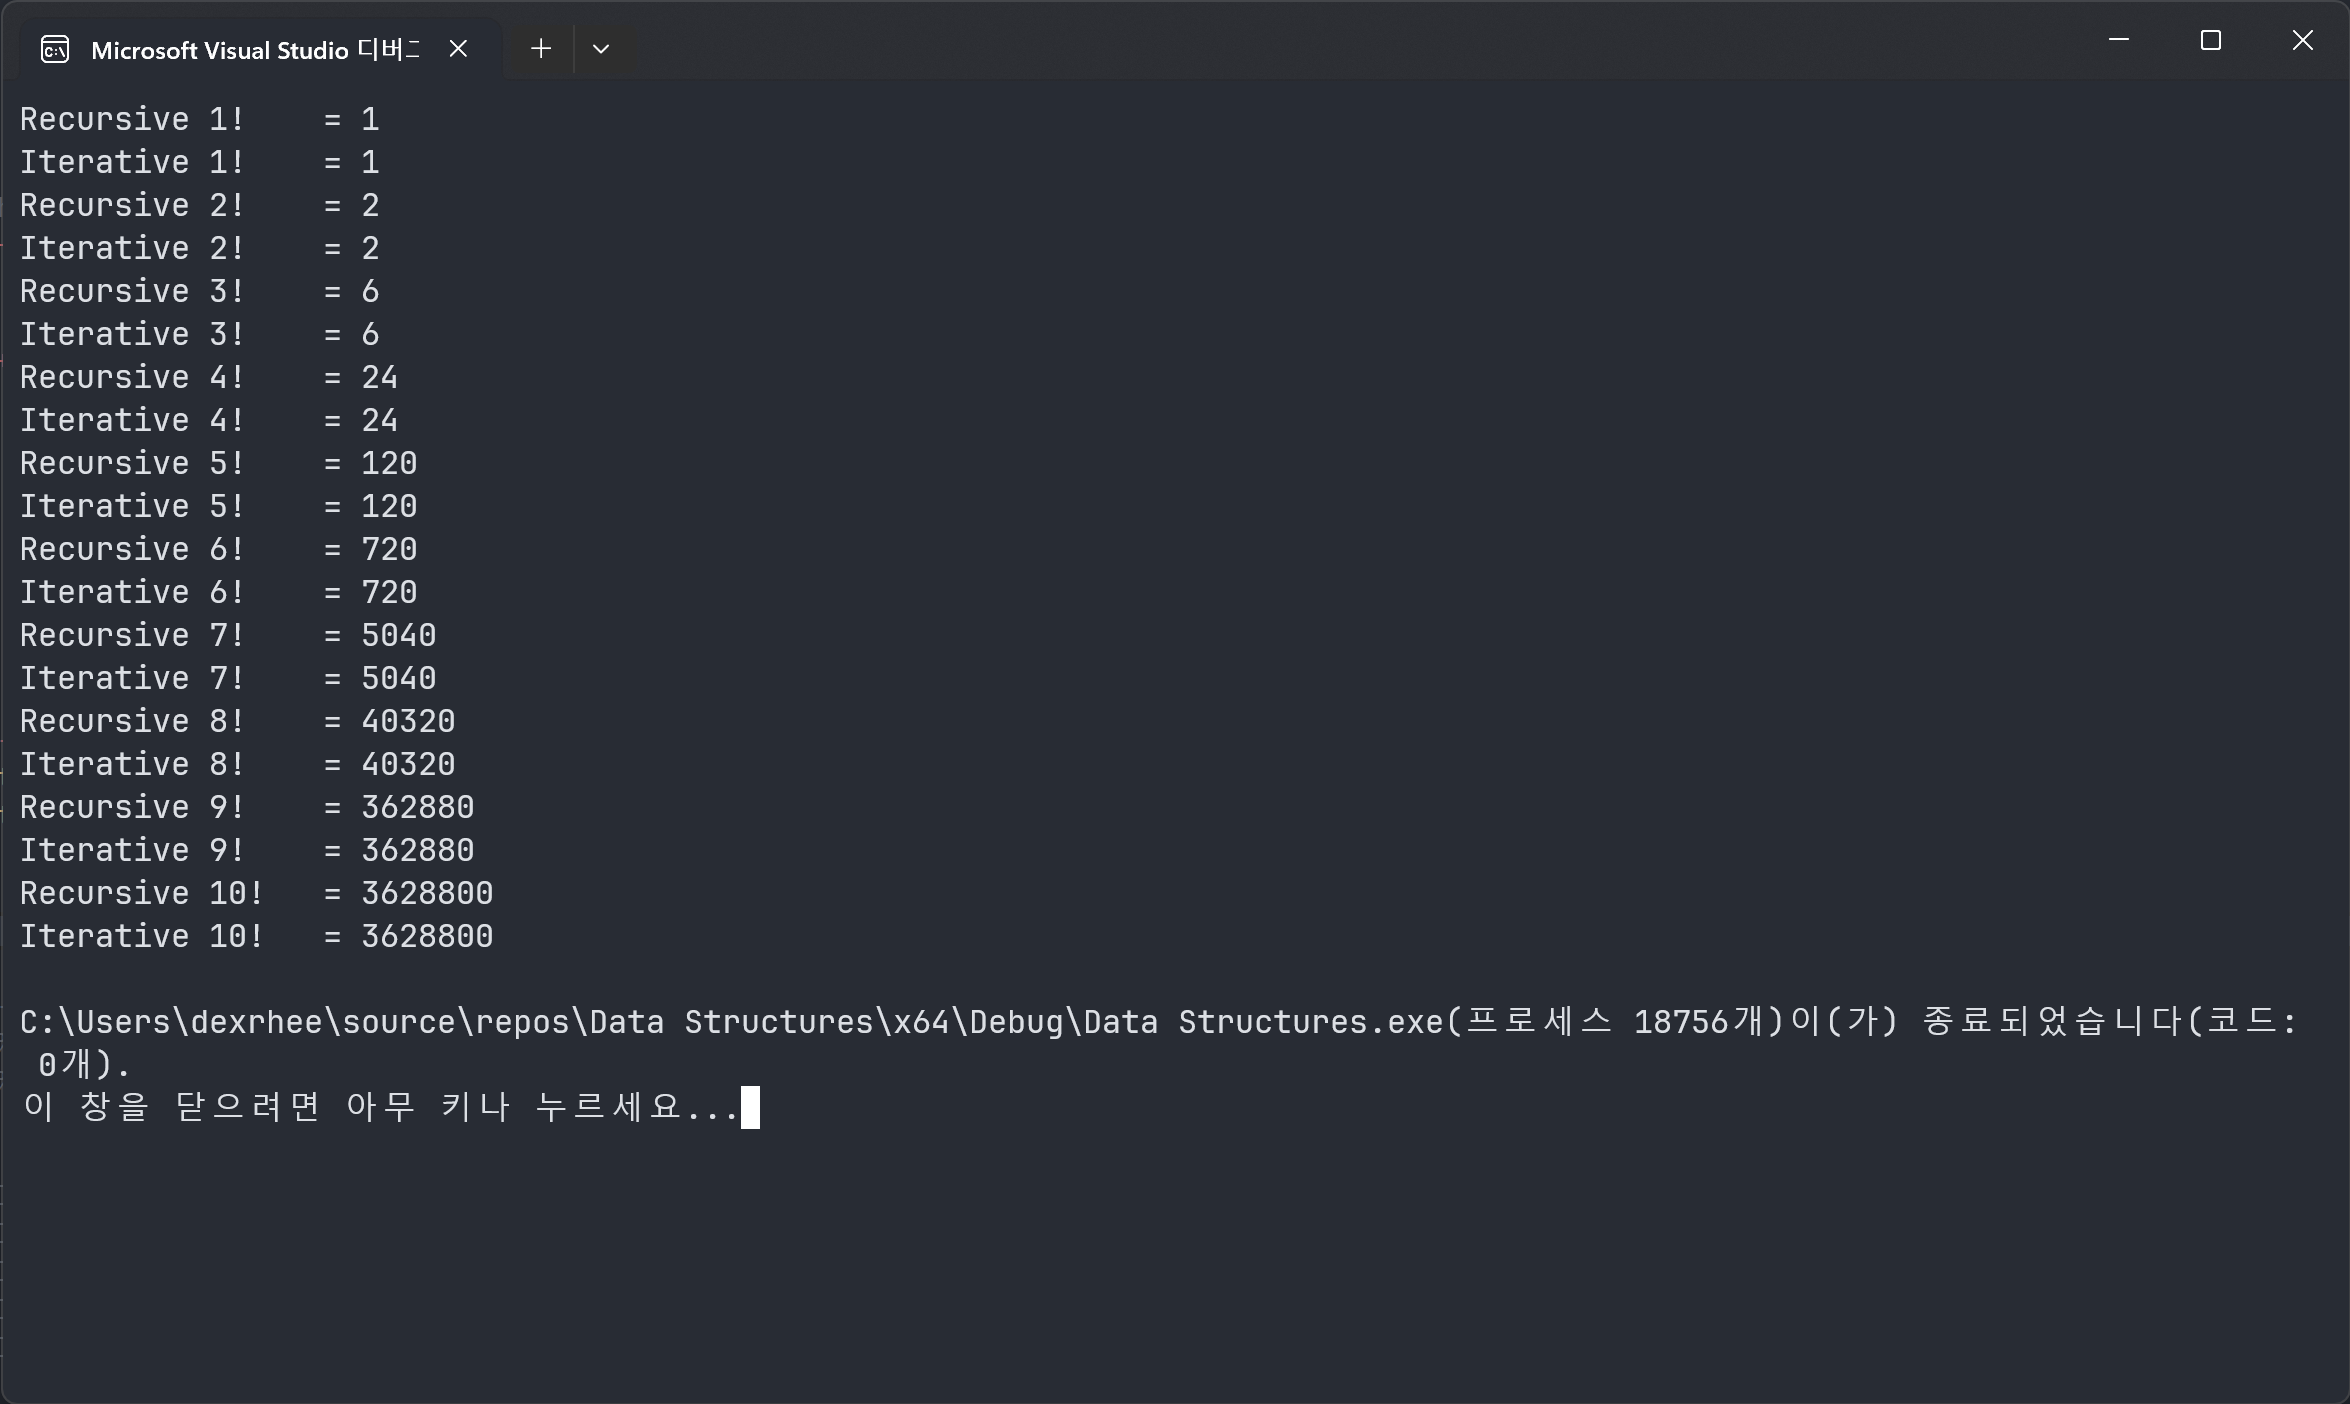
\includegraphics[width=\textwidth]{./img/1.png}
\newpage
\subsubsection{Problem 2}
피보나치 수열에 대한 프로그램도 recursion version과 iteration version을 각각 구현하고,
입력 값을 1-10까지 증가시키면서 화면에 출력되게 실행하시오.
(의도: 구현이 정확하게 되었는지를 보는 문제입니다.)

\paragraph{Solution.}
다음은 recursion version과 iteration version으로 fibonacci function을 구현한 소스코드입니다. (제출한 파일의 24-29번 라인)
\begin{minted}{c}
// 2-1. Recursive Version of the Fibonacci
int fibonacciRecursive(int n) {
    return n == 0 || n == 1 ?
        n :
        fibonacciRecursive(n - 2) + fibonacciRecursive(n - 1);
}

// 2-2. Iterative Version of the Fibonacci
int fibonacciIterative(int n) {
    int a = 0, b = 1, c;
    if (n == 0) return a;
    for (int i = 2; i <= n; i++) {
        c = a + b;
        a = b;
        b = c;
    }
    return b;
}
\end{minted}
위 함수의 parameter \texttt{n}을 1부터 10까지 증가시키며 테스트하기 위해 사용한 코드는 다음과 같습니다. (제출한 파일의 51-55번 라인)
\begin{minted}{c}
// 2-3. Fibonacci 1 to 10
    for (int i = 1; i <= 10; i++) {
    printf("Recursive fib(%d)\t= %d\n", i, fibonacciRecursive(i));
    printf("Iterative fib(%d)\t= %d\n", i, fibonacciIterative(i));
}
\end{minted}
\newpage
위의 코드를 실행한 결과는 다음과 같습니다.

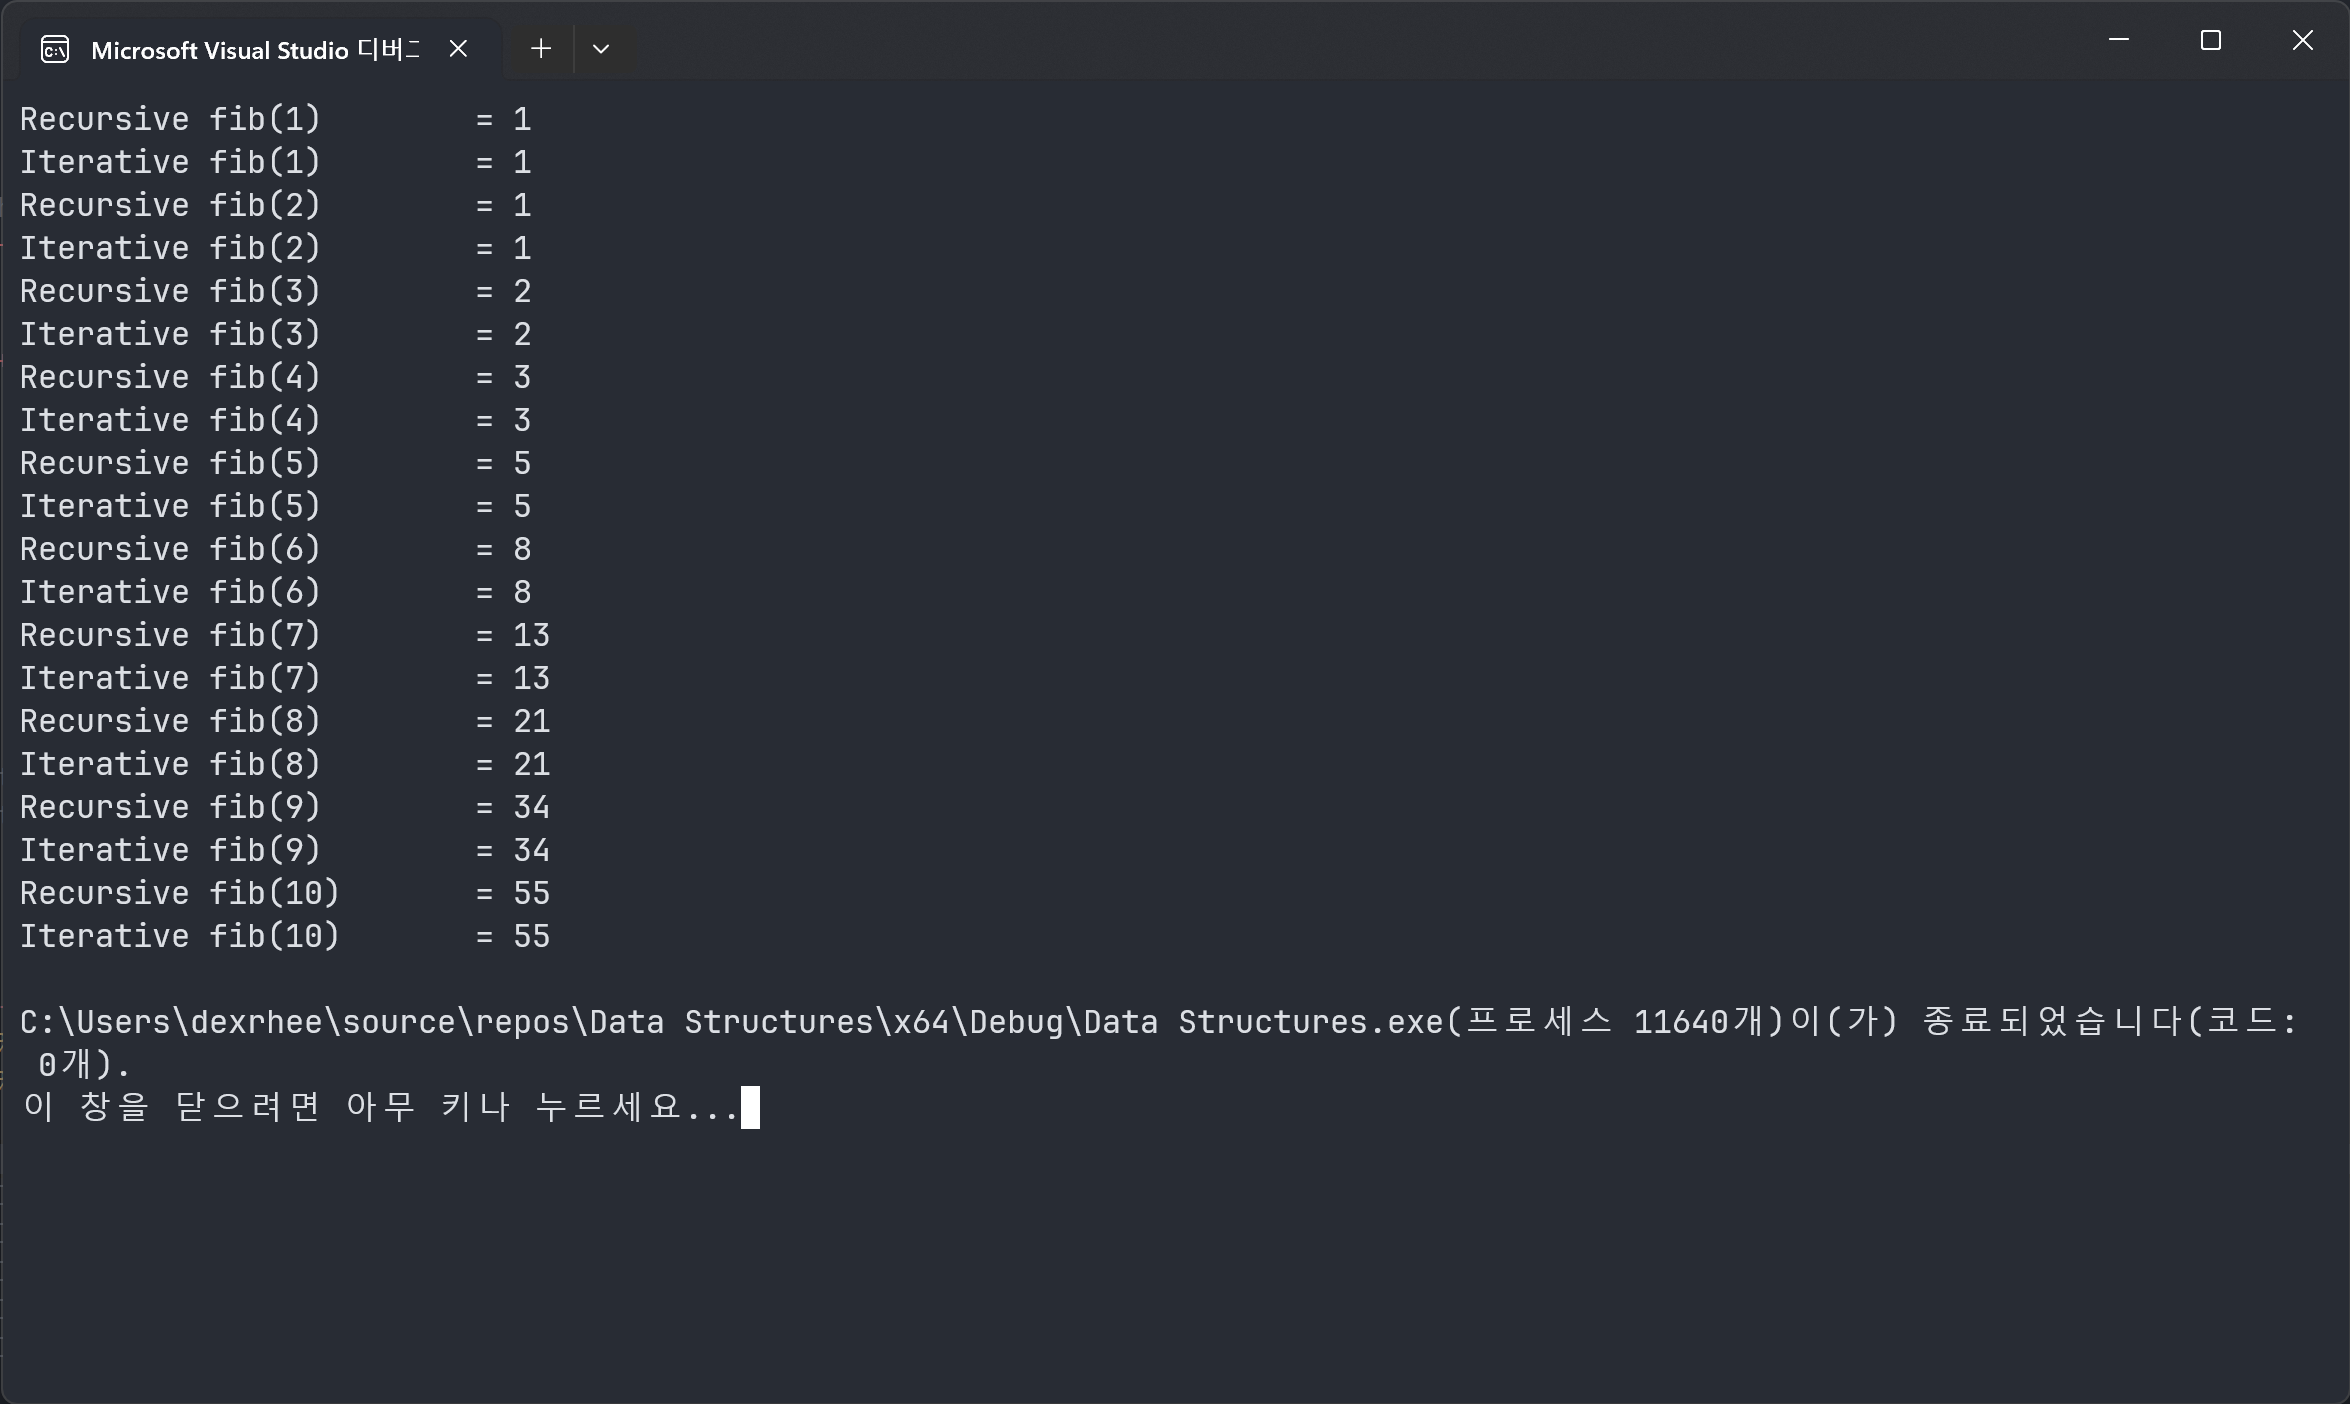
\includegraphics[width=\textwidth]{./img/2.png}
\newpage
\subsubsection{Problem 3}
Factorial recursion version의 경우,
\texttt{n}이 증가함에 따라
어느 정도의 \texttt{n}에서까지는 실행(예, 1000, 2000, 3000, 4000. 수행 컴퓨터마다 다를 수 있음)이 잘 되지만,
어느 정도 이후(약 5000. OS따라 Compiler에 따라 한계값이 다를 수 있음)에는
``stack overflow''로 수행이 안 됨을 보이시오.
단, \texttt{factorial(1000)}등은 결과값이 너무 커서,
그 결과값을 \mintinline{c}|unsigned long long| 타입으로 설정하여도 overflow됨으로 결과값은 틀려도 됩니다.
(의도: stack overflow 로 인해 run time error로 수행이 멈춘다는 것을 확인하는 것입니다.)

\paragraph{Solution.}
위 상황을 테스트하기 위해 사용한 코드는 아래와 같습니다. (제출한 파일의 57-60번 라인)
\begin{minted}{c}
// 3, 5. Testing Stack Overflow with Recursive Function
for (int i = 1; i < 10000; i *= 2) {
    printf("%d!\t= %lld\n", i, factorialRecursive(i));
}
\end{minted}
위 코드는 \mintinline{c}|factorialRecursive| 함수의 파라미터 \texttt{n} 값을 1부터 시작해 2씩 곱하며 10,000 전 까지의 수(이 경우 8,192까지) 모두를 테스트 하는 코드입니다.
위의 코드를 실행한 결과는 다음과 같습니다.

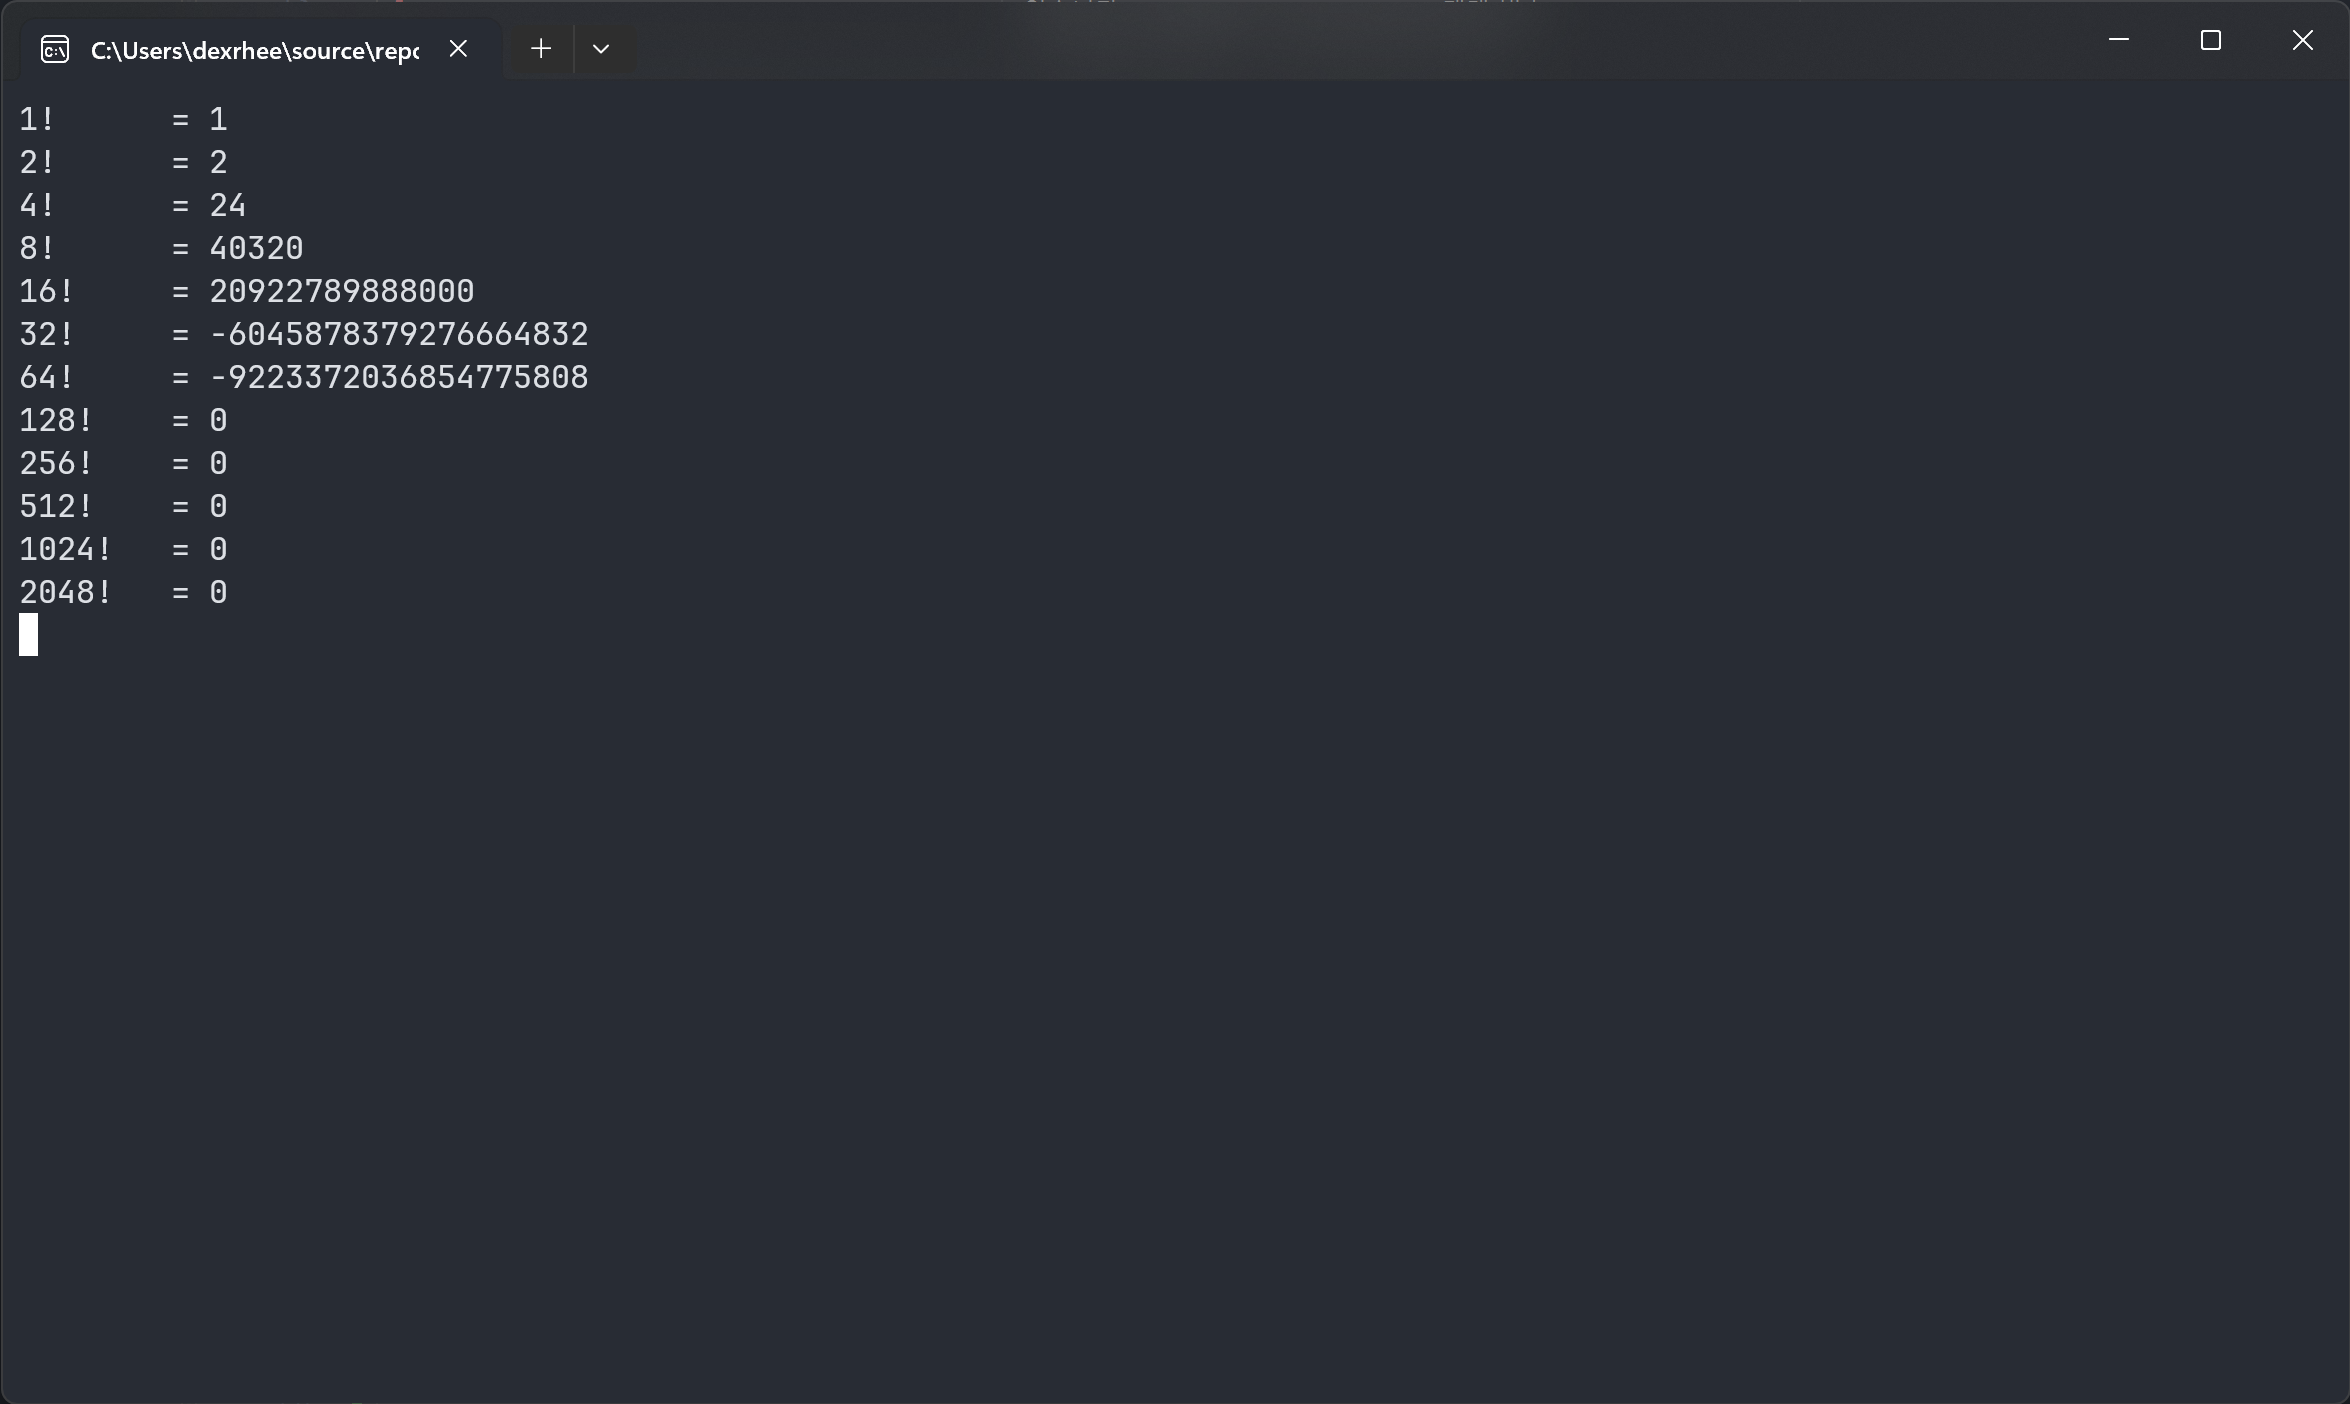
\includegraphics[width=\textwidth]{./img/3-1.png}
Output을 확인해보면, \texttt{n}의 값이 작을 경우 값이 정상적으로 표현되나,
\texttt{factorialRecursive} 함수의 Return type인 \mintinline{c}|long long|의 범위를 초과하는 수에 대해서는 Overflow가 일어나 정상적인 값이 표현되지 않는 것을 볼 수 있습니다.
또한, \mintinline{c}|factorialRecursive(2048)|의 값 까지는 정상적으로 출력되지만, 이후의 값은 나타나지 않는 모습을 확인할 수 있습니다.

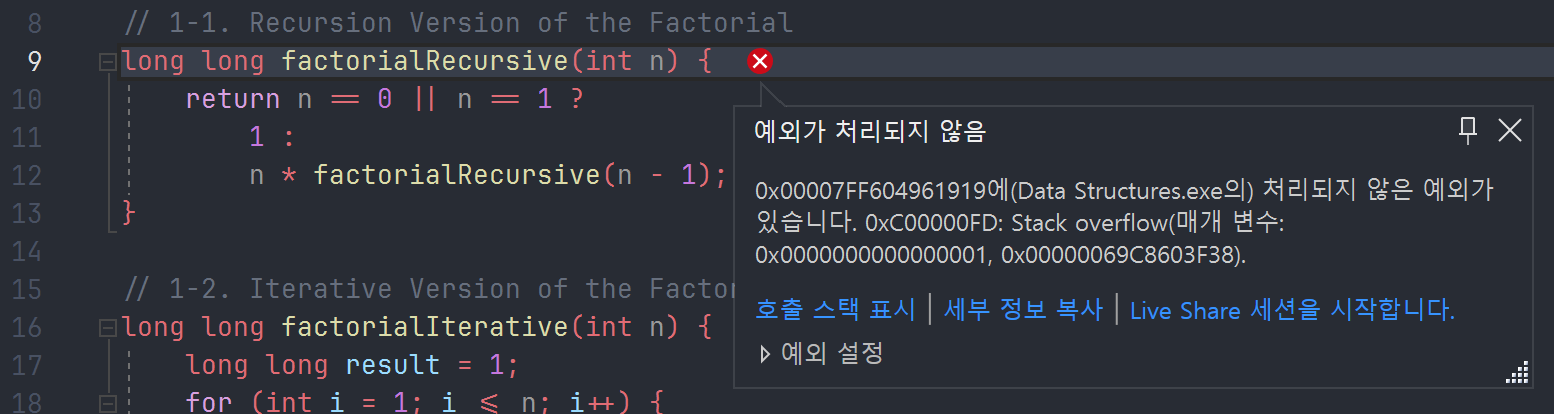
\includegraphics[width=\textwidth]{./img/3-2.png}
Visual Studio의 Debug 도구를 사용하여 왜 2048 이후의 값이 출력되지 않았는지 확인해보면,
Stack Overflow가 발생하여 run time error로 수행이 멈추었다는 것을 확인할 수 있습니다.

\subsubsection{Problem 4}
하지만, 이 경우(\texttt{n = 5000})에도 iteration version은 실행이 잘 됨을 보이시오.
이 경우도 결과 값은 틀려도 됩니다.
(의도: loop이 끝까지 동작해서, 만약 결과값만 잘 담을 수 있는 방법이 있다면 실행이 가능함을 확인하는 것입니다.)

\paragraph{풀이} 위 상황을 테스트하기 위해 사용한 코드는 아래와 같습니다. (제출한 파일의 62-65번 라인)
\begin{minted}{c}
for (int i = 1; i < 10000; i *= 2) {
    printf("%d!\t= %lld\n", i, factorialIterative(i));
}
\end{minted}
위 코드는 \mintinline{c}|factorialIterative| 함수의 파라미터 \texttt{n} 값을 1부터 시작해 2씩 곱하며 10,000 전 까지의 수(이 경우 8,192까지) 모두를 테스트 하는 코드입니다.
위의 코드를 실행한 결과는 다음과 같습니다.

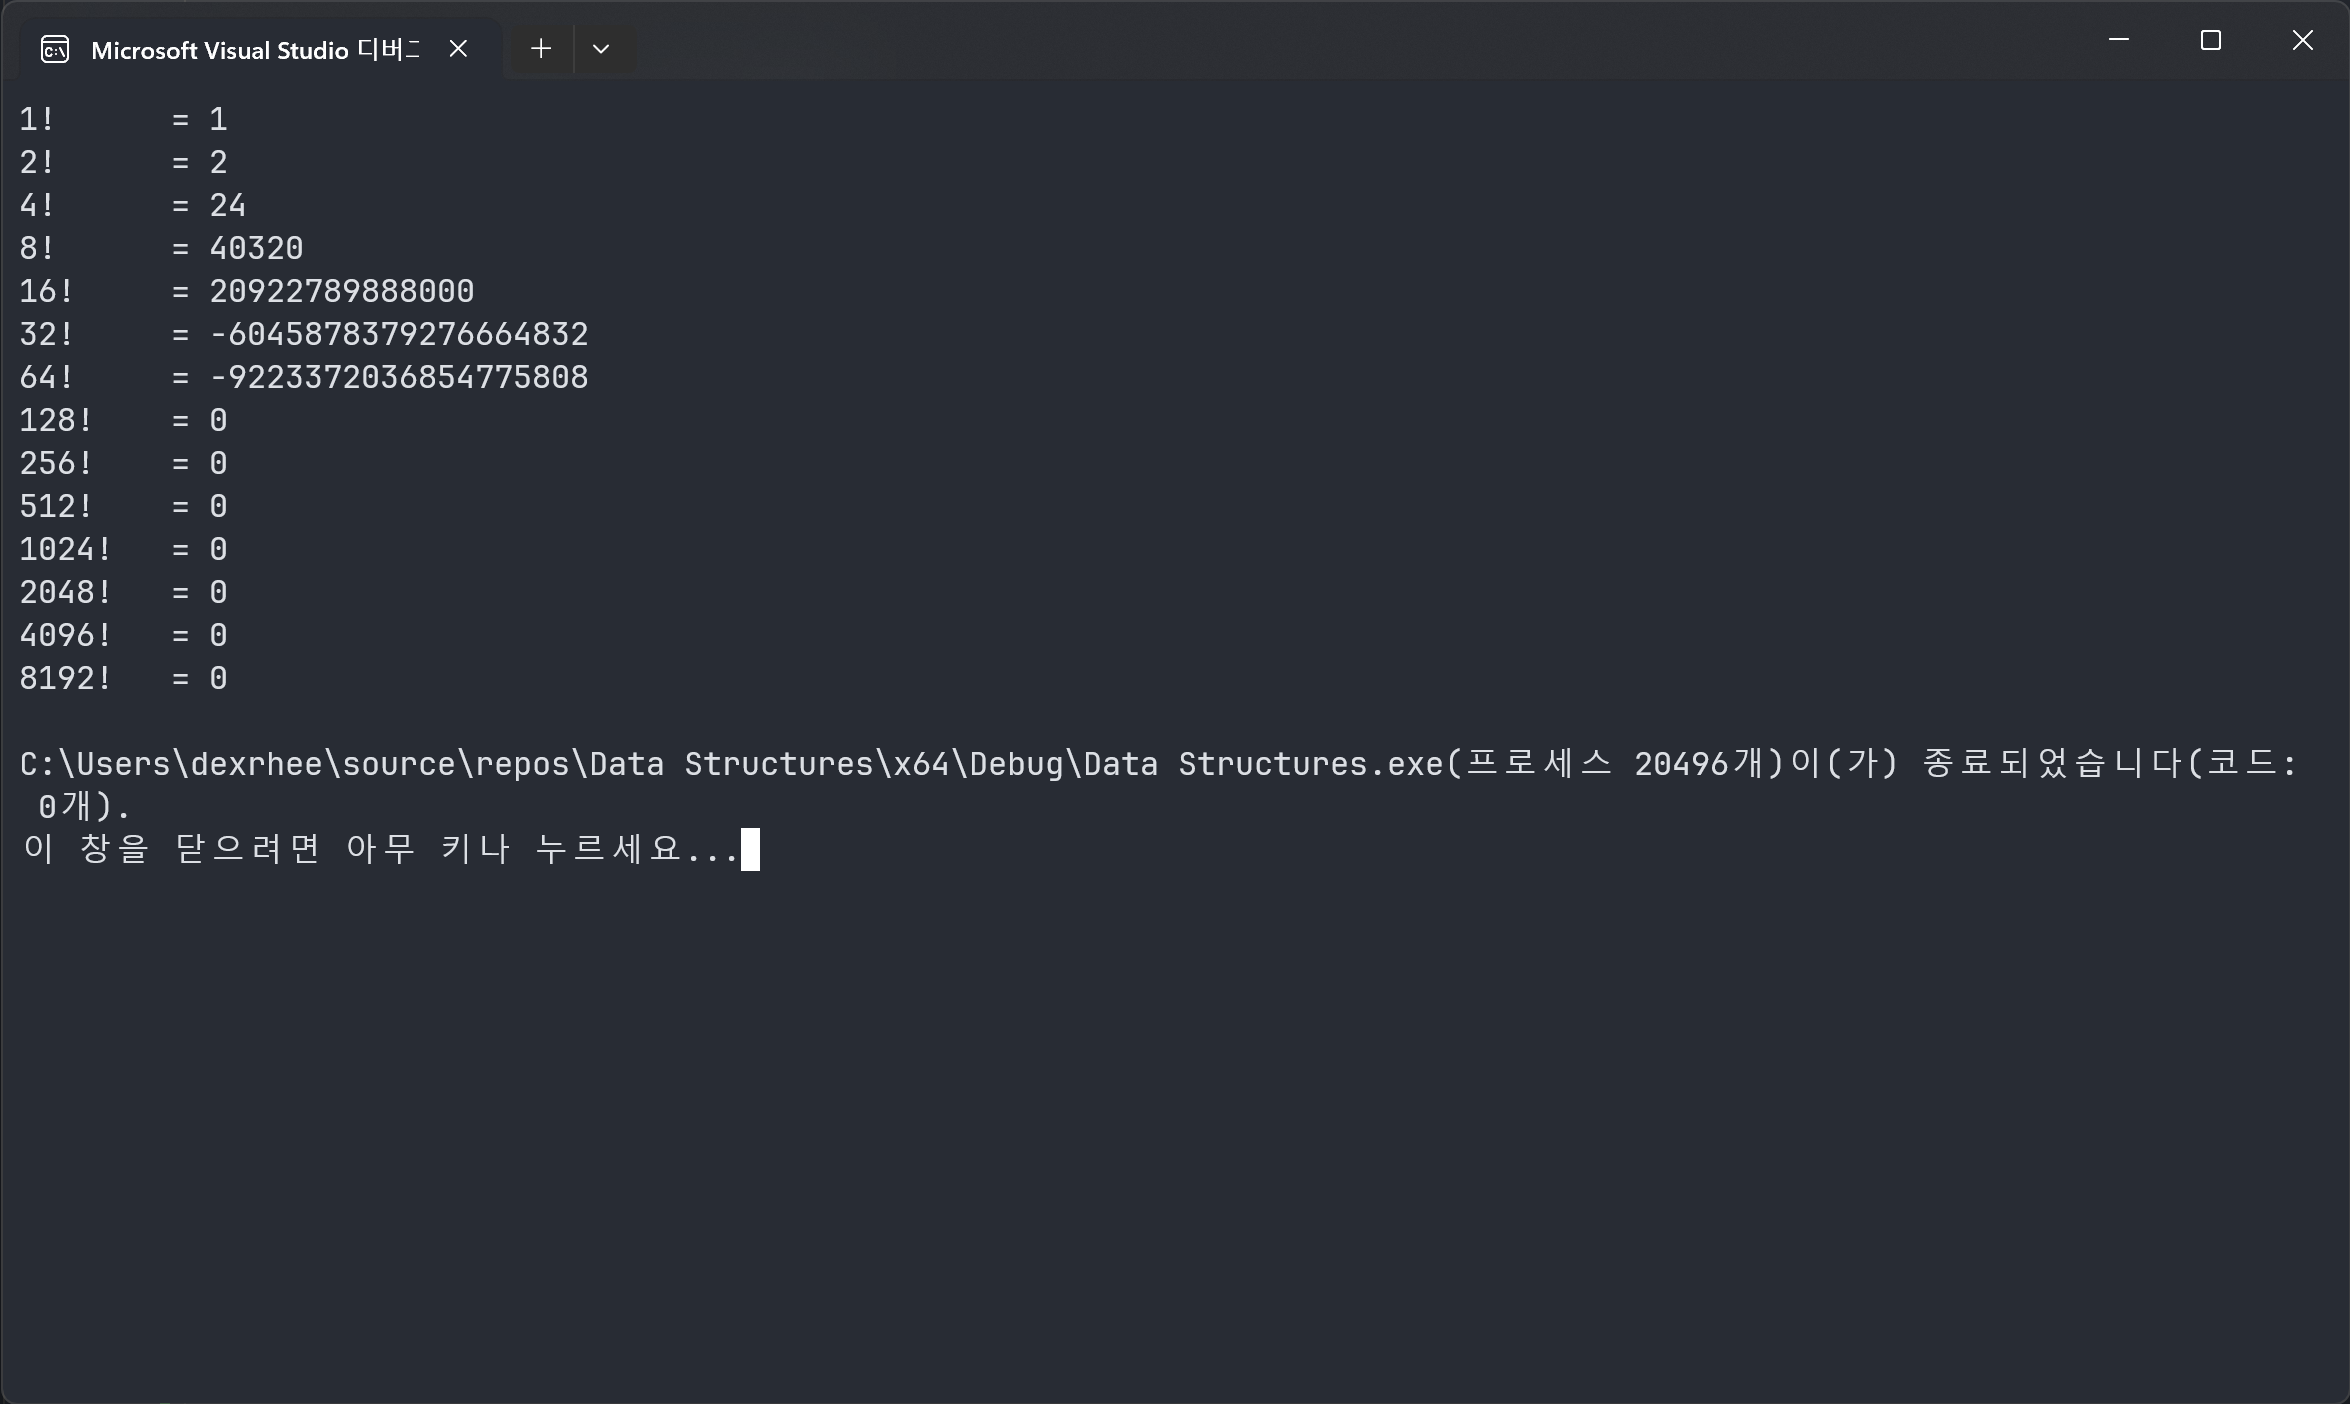
\includegraphics[width=\textwidth]{./img/4.png}

\texttt{factorialRecursive} 함수의 Return type인 \mintinline{c}|long long|의 범위를 초과하는 수에 대해서는 Overflow가 일어나 정상적인 값이 표현되지 않는 것을 볼 수 있습니다.
또한, Recursion version과는 다르게, \mintinline{c}|factorialIterative(2048)| 이후의 값도 정상적으로 출력되는 것을 확인할 수 있습니다.
\subsubsection{Problem 5}
\subsubsection{(1)}
프로그램이 프로세스로서 실행될 때, 구성되는 메모리 공간에 대해서 조사하시오.
(즉, 코드영역, Data영역, Heap 영역, Stack 영역)

\paragraph{Solution.}
프로그램이 실행되기 위해서는, OS가 프로그램의 정보를 메모리에 로드해야합니다.
또한 프로그램이 실행되는 동안 CPU가 코드를 처리하기 위해 메모리가 명령어와 데이터들을 저장해야합니다.
이렇게 프로그램이 OS로 부터 할당받는 대표적인 메모리 공간은 Code 영역, Data 영역, Heap 영역, Stack 영역으로 구성되어 있습니다.

Code 영역은 실행할 프로그램의 코드가 저장되는 영역으로,
CPU는 코드 영역에 저장된 명령을 하나씩 가져가 처리합니다.
저장된 프로그램의 코드는 프로그램이 시작하고 종료될 때까지 메모리에 계속 남아있는다.

Data 영역은 프로그램의 Global 변수와 Static 변수가 저장되는 영역으로,
프로그램의 시작과 함께 할당되며 프로그램이 종료되면 소멸합니다.

Heap 영역은 프로그래머가 직접 공간을 할당, 해제하는 메모리 공간입니다.
Heap 영역에서 공간을 할당, 해제받을 수 있는 C언어의 대표적인 방법으로는, \mintinline{c}|malloc()|, \mintinline{c}|free()|가 있습니다.
Heap 영역은 메모리의 낮은 주소에서 높은 주소의 방향으로 할당되기 떄문에, FIFO\textsuperscript{First-In First-Out} 구조입니다.

Stack 영역은 프로그램이 자동으로 사용하는 임시 메모리 영역입니다.
함수 호출 시 생성되는 지역 변수와 매개 변수가 저장되는 영역이고, 함수 호출이 완료되면 사라집니다.
이때 Stack 영역에 저장되는 함수의 호출 정보를 Stack Frame 이라고 합니다.
Stack 영역은 메모리의 높은 주소에서 낮은 주소의 방향으로 할당 되기 때문에, LIFO\textsuperscript{Last-In First-Out} 구조입니다.
\newpage
\subsubsection{(2)}
그리고, Visual studio (또는 본인이 사용 하는 개발 환경)에서 Stack 영역의 크기를 조정하여,
위 3번 문제의 실행될 수 있는 한계가 달라짐을 보이시오.

\paragraph{Solution.}
Visual Studio에서 Stack의 크기를 조정하려면, 프로젝트 > 속성 > 링커 > 시스템에서 스택 예약 크기를 변경하면됩니다.

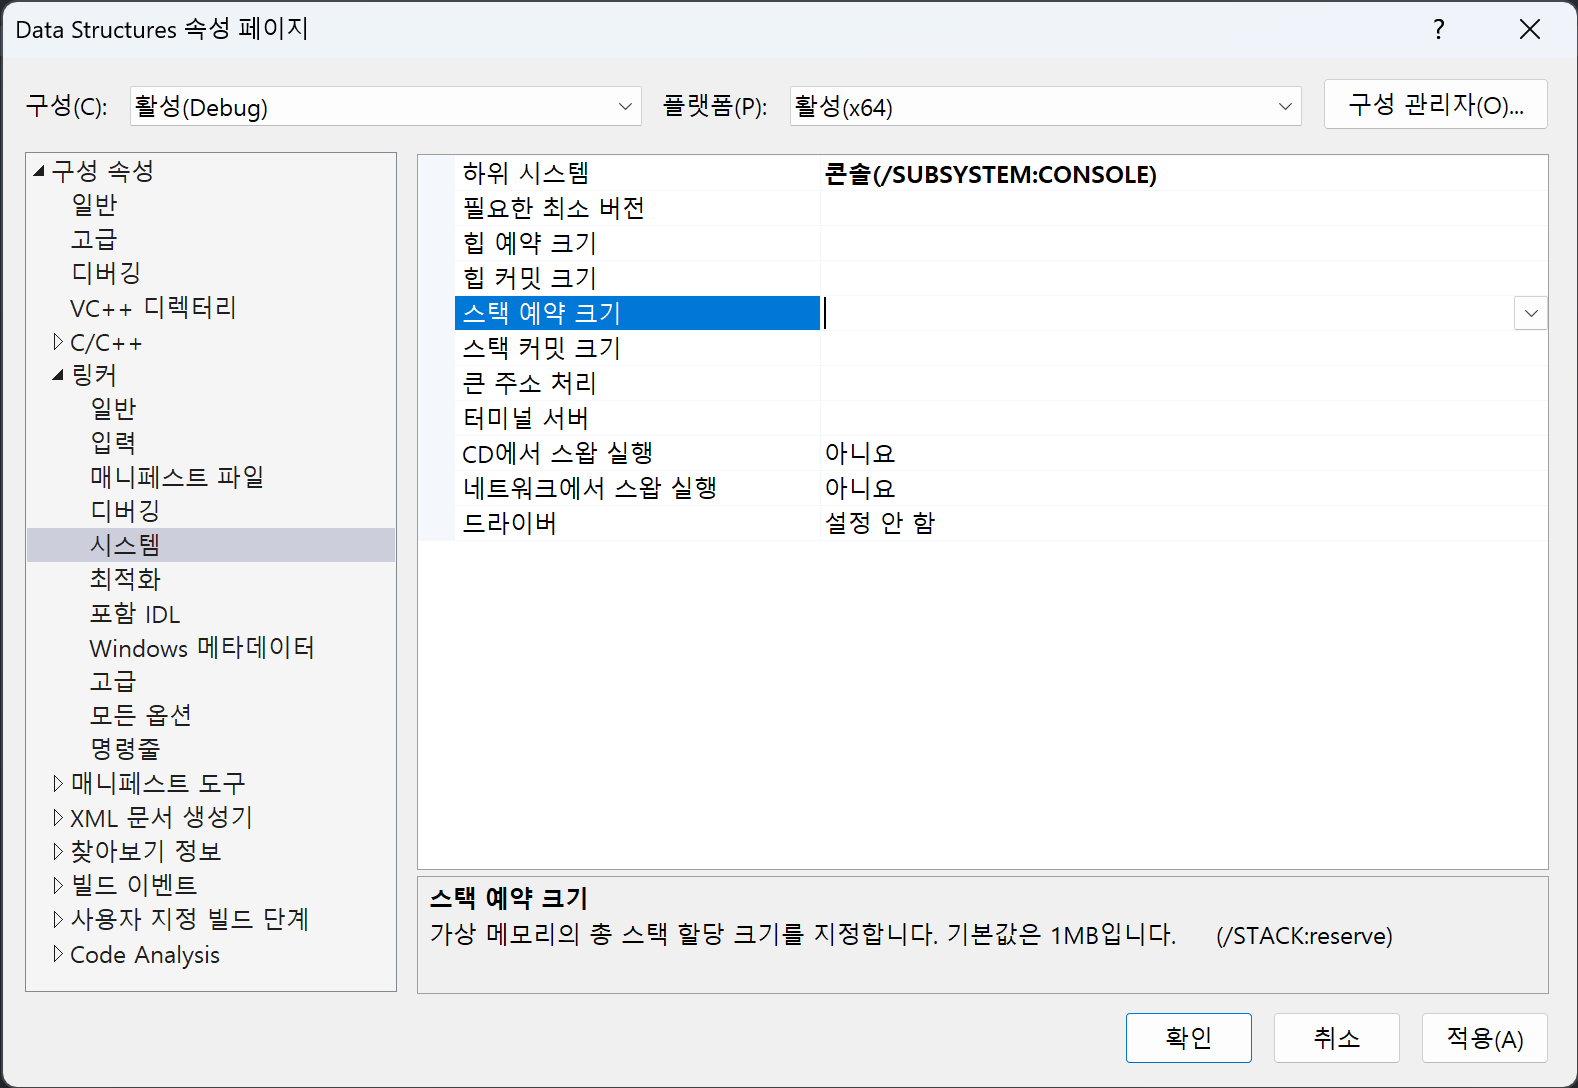
\includegraphics[width=\textwidth]{./img/5-1.png}
Visual Studio에서의 기본 Stack Size는 1MB($2^20$B = 1,048,576B)이므로, 이와 다른 값을 적절히 지정해주면 위 3번 문제의 실행에 유의미한 변화를 볼 수 있을 것입니다.

\paragraph{Case 1.} Stack Size를 1KB = 1,024B로 설정한 경우

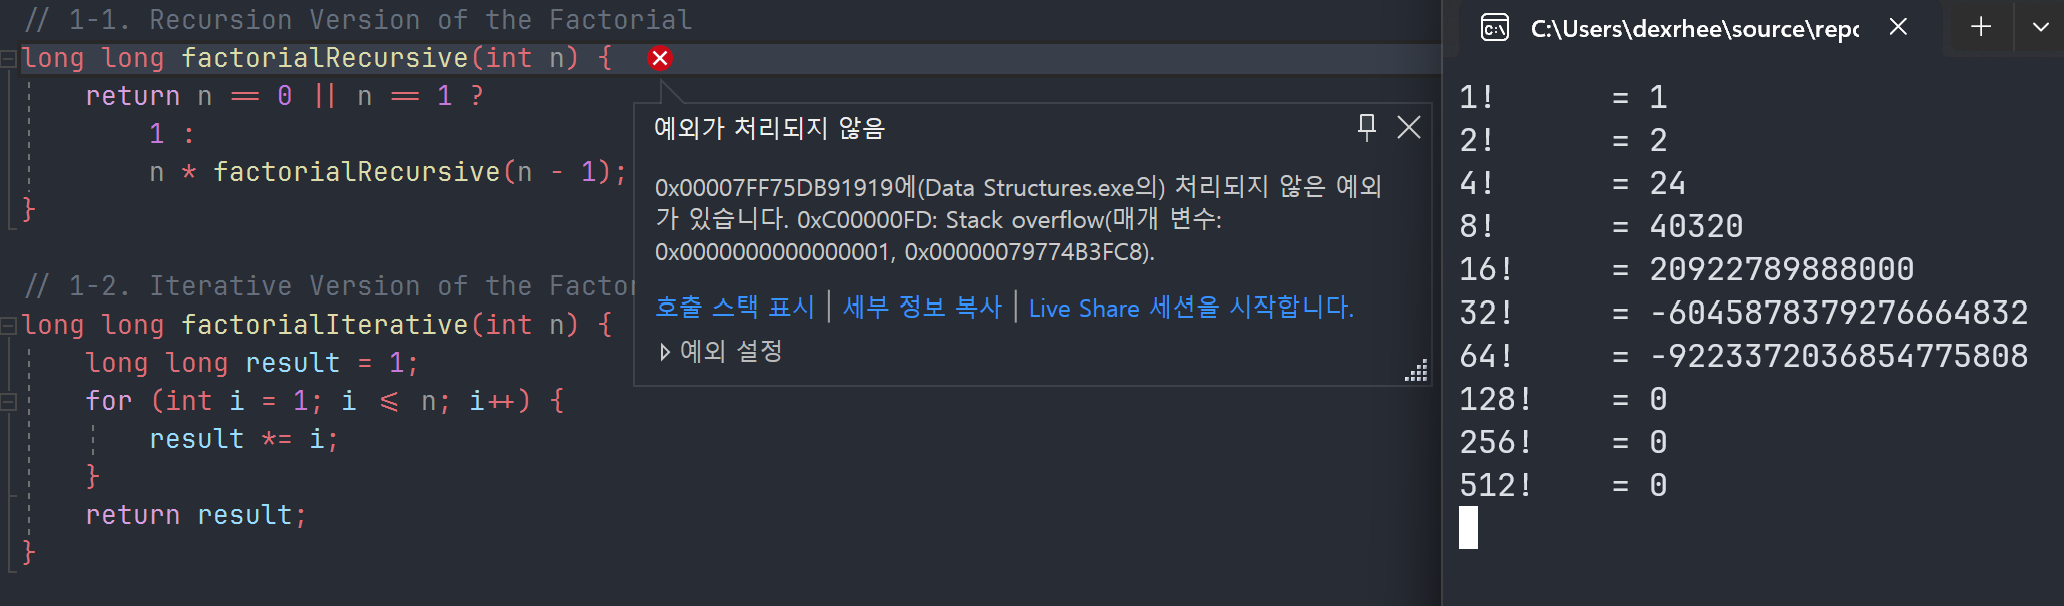
\includegraphics[width=\textwidth]{./img/5-2.png}
위 3번에서 실행한 코드와 동일한 코드를 1,024B의 Stack Size를 가지고 실행했을 경우,
위의 그림에서 볼 수 있듯 \mintinline{c}|factorialRecursive(512)|까지는 정상 실행되지만,
\mintinline{c}|factorialRecursive(1024)|부터 Stack Overflow가 발생하는 것을 볼 수 있습니다.

\paragraph{Case 2.} Stack Size를 10MB = 10,485,760B로 설정한 경우

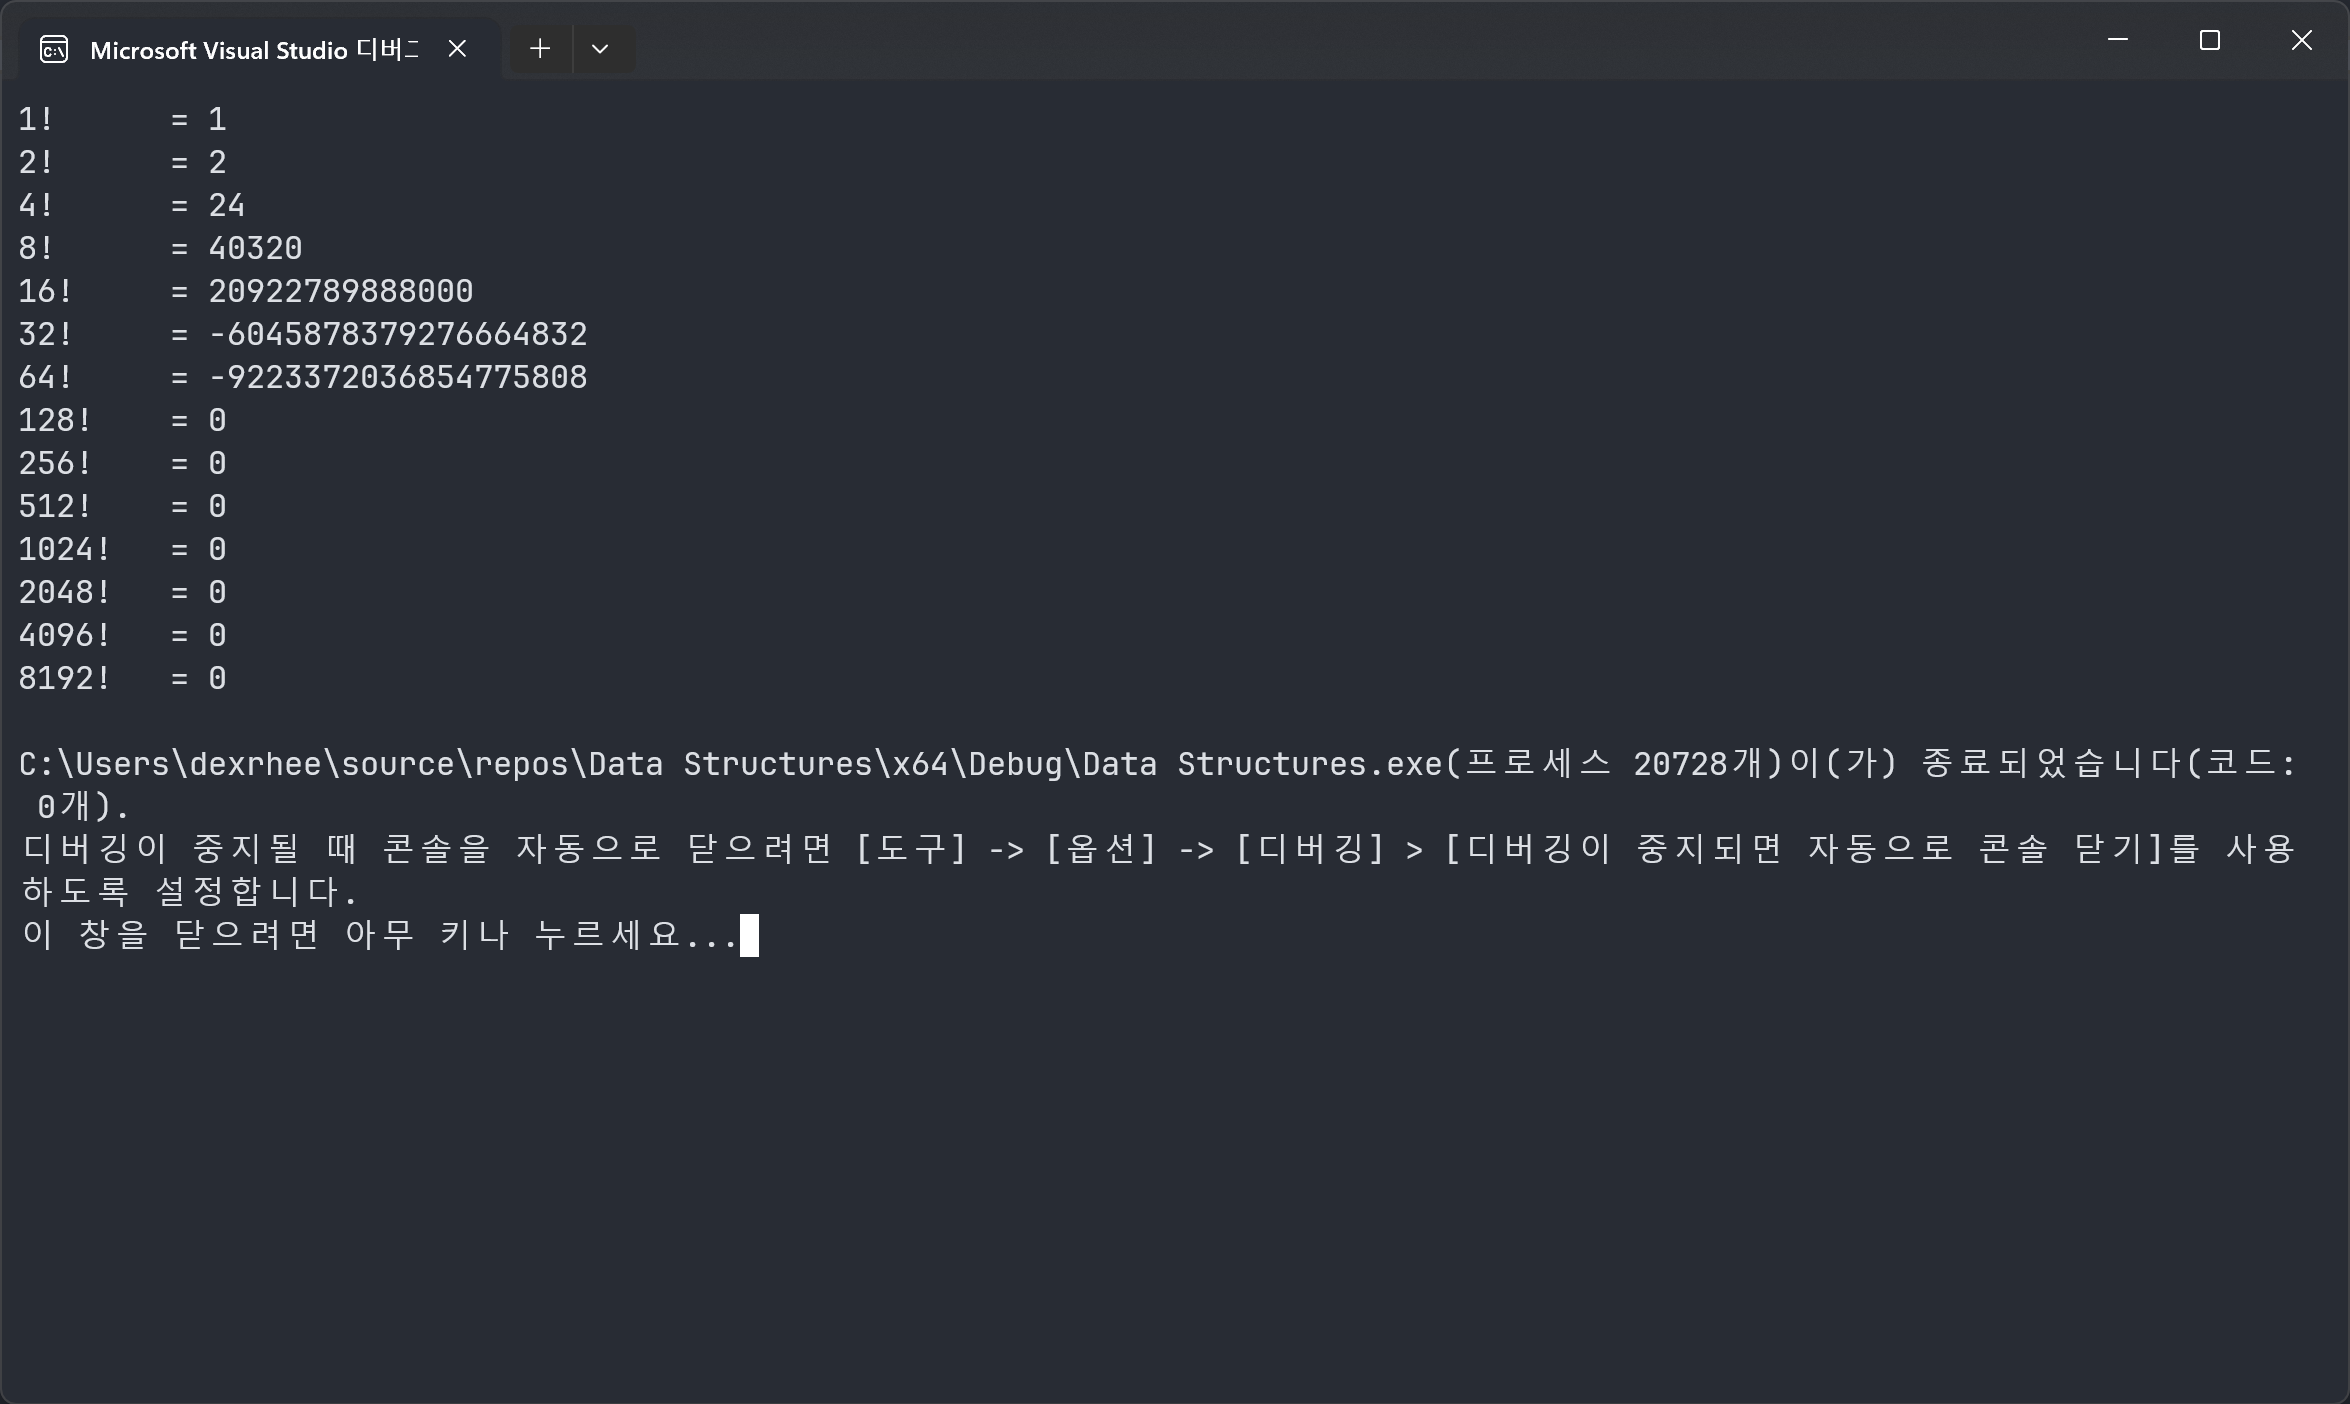
\includegraphics[width=\textwidth]{./img/5-3.png}
위 3번에서 실행한 코드와 동일한 코드를 10MB의 Stack Size를 가지고 실행했을 경우,
위의 그림에서 볼 수 있듯 \mintinline{c}|factorialRecursive(8192)|까지 모두 실행되고,
정상적으로 프로그램이 종료되었음(Exit code가 0임)을 확인할 수 있습니다.

\subsubsection{(3)}
Visual studio에는 컴파일 옵션이 디버그모드와 릴리즈모드가 있는데,
그 차이점을 조사하고, 위 3번 문제의 실험 결과가 두 가지 모드에서 다르게 나오는 것을 보이시오.

\paragraph{Solution.} Visual Studio에서 프로젝트를 Build 하는 방법에는 Release와 Debug의 두 가지 방식이 있습니다.
Release 모드와 Debug 모드는 컴파일러 최적화, 코드 실행 중 예외 처리, 코드의 안정성, 코드의 크기 면에서 차이가 있습니다.

먼저 컴파일러 최적화 면에서,
Debug 모드는 최적화를 거의 하지 않아서 디버깅 시 변수의 값을 추적하기 쉽습니다.
반면에 Release 모드는 최적화를 많이 하기 때문에 실행 속도가 빨라집니다. 하지만 디버깅 시 변수 추적이 어렵습니다.

코드 실행 중 예외 처리 면에서,
Debug 모드는 발생한 예외를 즉시 보고하고, 디버거를 통해 프로그램의 상태를 쉽게 파악할 수 있습니다.
반면에 Release 모드는 발생한 예외를 적절히 처리하고, 프로그램이 멈추는 것을 방지합니다. 하지만 예외가 발생한 위치를 찾기 어렵습니다.

코드의 안정성 면에서,
Debug 모드는 코드의 안정성을 위해 추가적인 검사와 확인을 수행합니다.
반면에 Release 모드는 실행 속도를 위해 검사를 줄이기 때문에, 더 적은 검사를 수행하고 실행 속도를 빠르게 합니다.

코드의 크기 면에서,
Debug 모드는 디버깅을 위해 많은 정보를 포함하고 있기 때문에 코드 크기가 큽니다.
반면에 Release 모드는 최적화를 많이 하기 때문에 코드 크기가 작아집니다.

요약하면, Debug 모드는 디버깅과 코드 안정성에 중점을 두고, Release 모드는 실행 속도와 코드 크기에 중점을 두는 것입니다.
따라서, 개발 시에는 Debug 모드로 작업하고, 배포 시에는 Release 모드로 컴파일하여 실행하는 것이 적합합니다.

위의 내용을 참고하여 두 가지 모드에 따라 실행 결과가 달라지는지 확인해보도록 합시다.
이전에 보았듯,
Debug 모드에서 위 3번의 코드를 실행하였을 때에는 다음의 그림과 같이 \mintinline{c}|factorialRecursive(2048)| 까지만 작동하고
\mintinline{c}|factorialRecursive(4096)|부터는 Stack Overflow가 발생함을 알 수 있습니다.

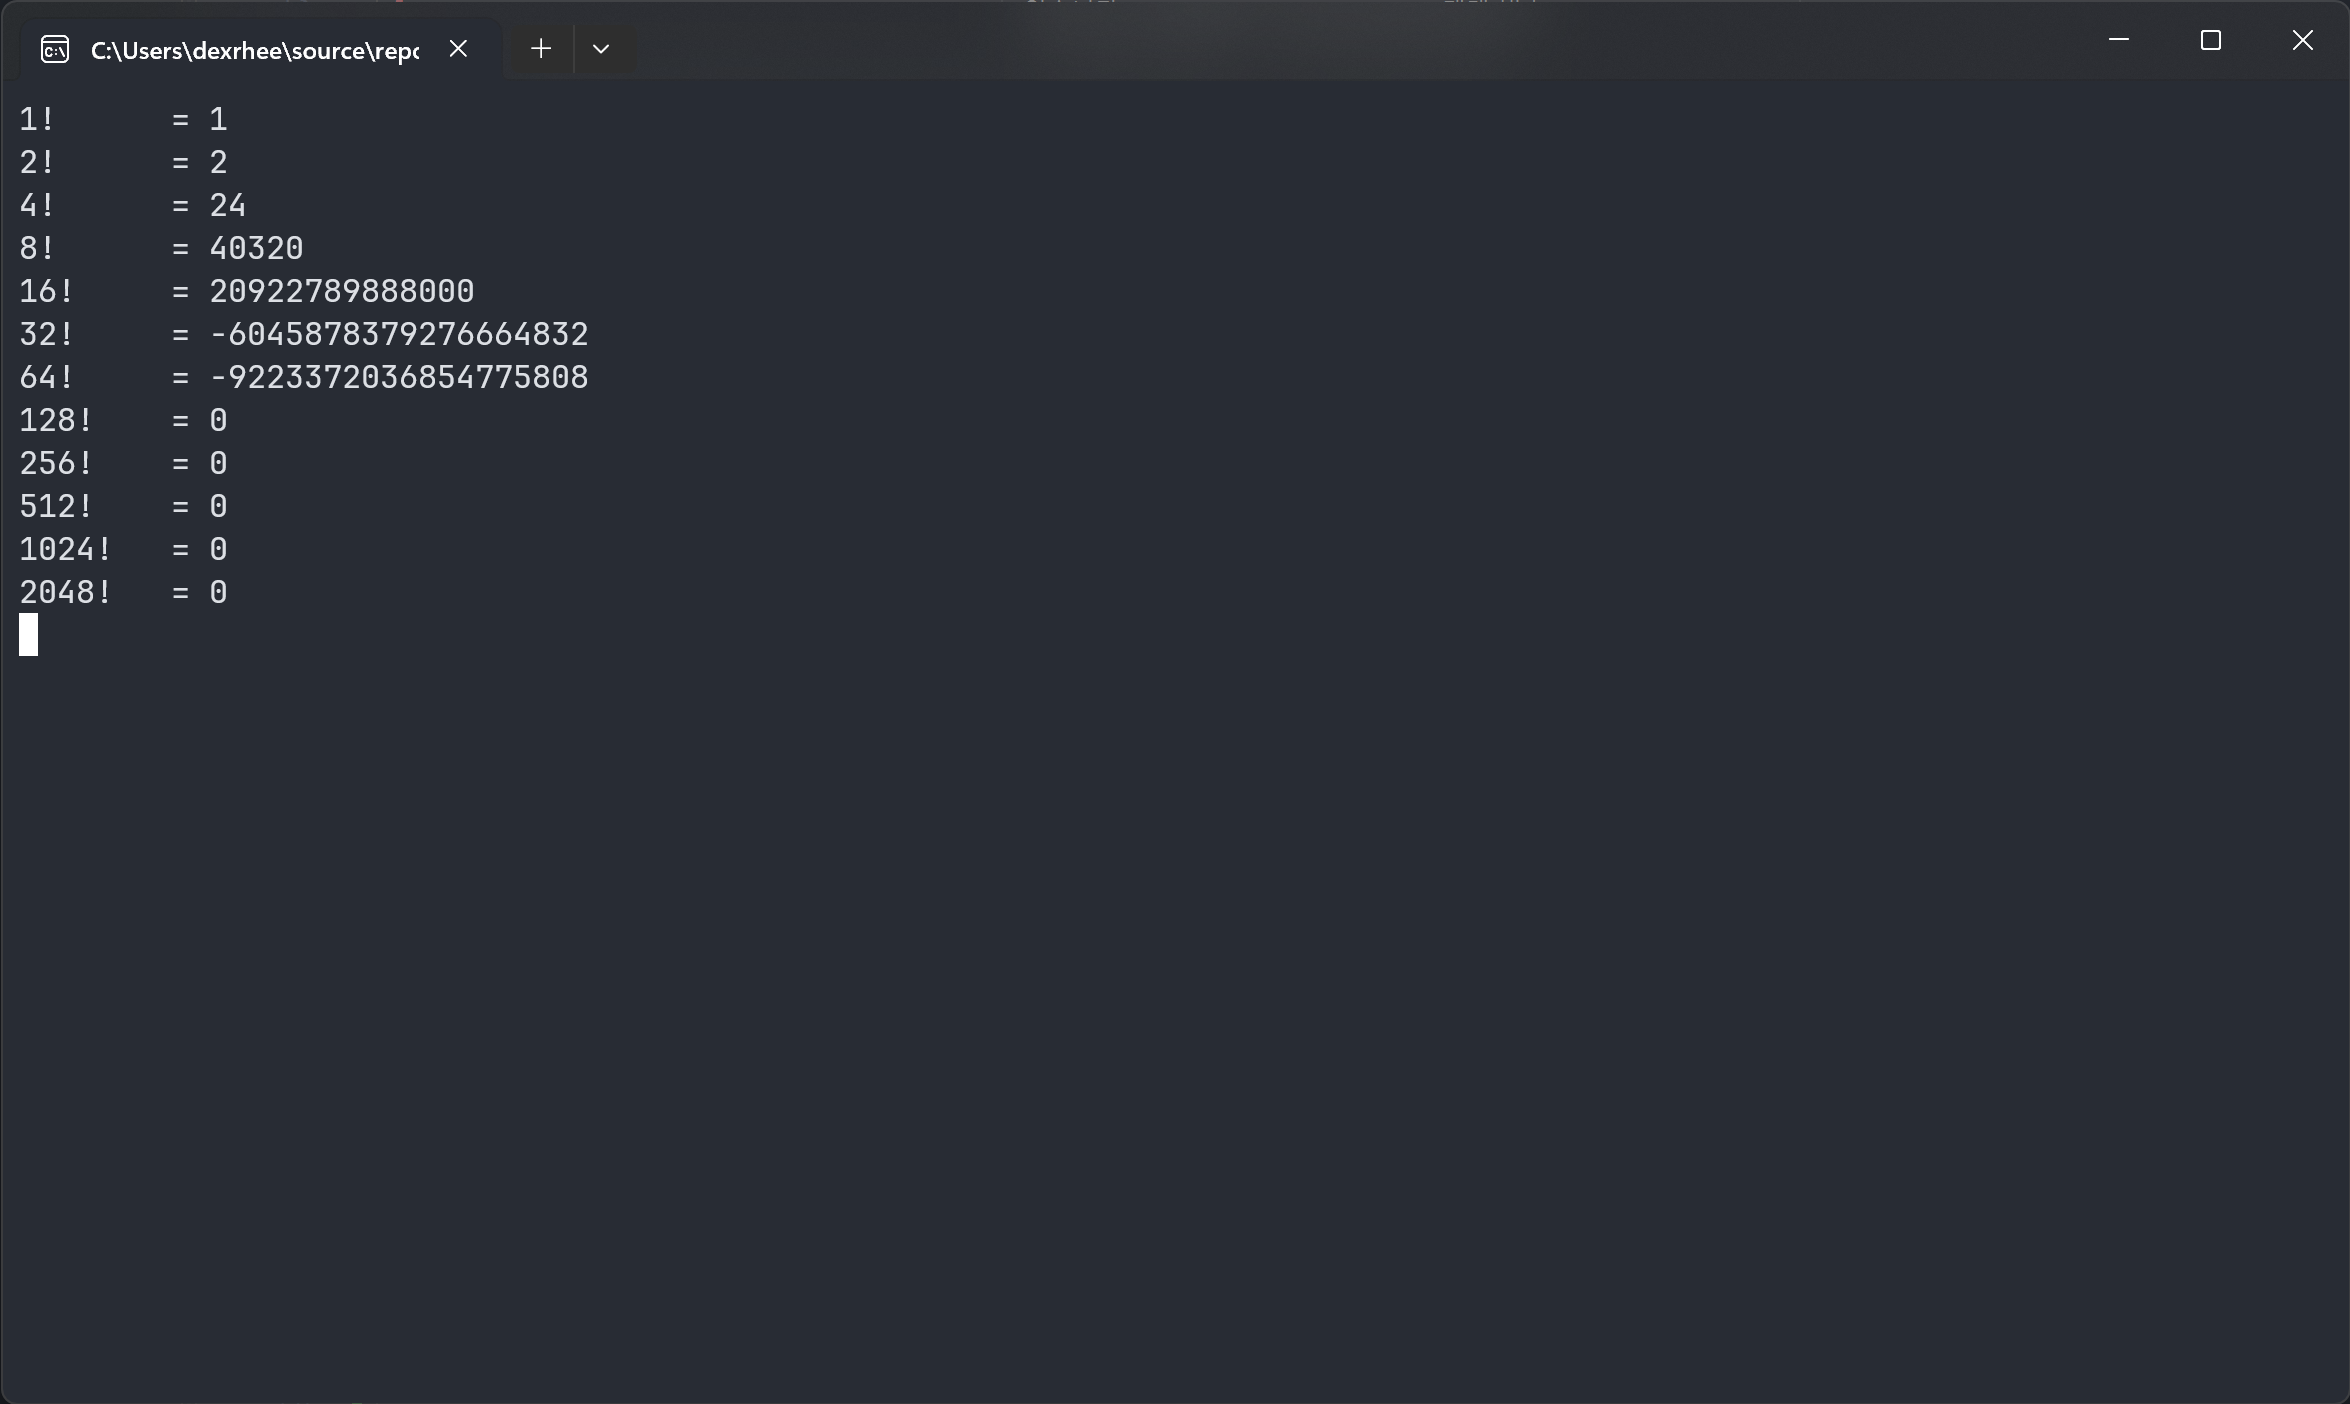
\includegraphics[width=\textwidth]{./img/3-1.png}
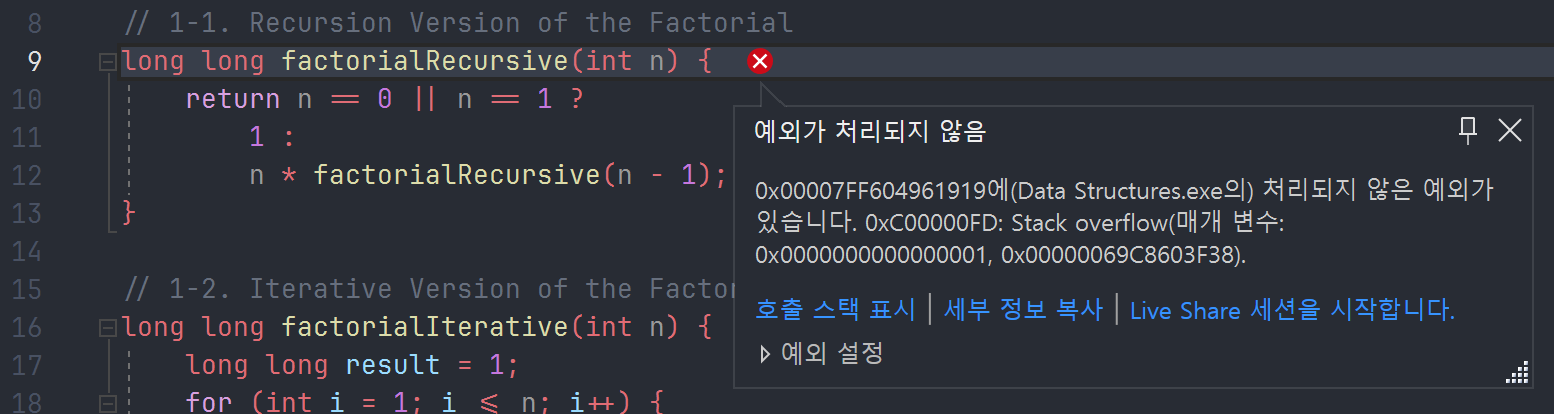
\includegraphics[width=\textwidth]{./img/3-2.png}

하지만 Release 모드로 프로젝트를 Build 후 실행하였을 때에는 다음의 그림과 같이 Stack Overflow가 발생하지 않고
\mintinline{c}|factorialRecursive(8192)|의 값까지 모두 출력되고 정상적으로 프로그램이 종료되었음(Exit code가 0임)을 확인할 수 있습니다.

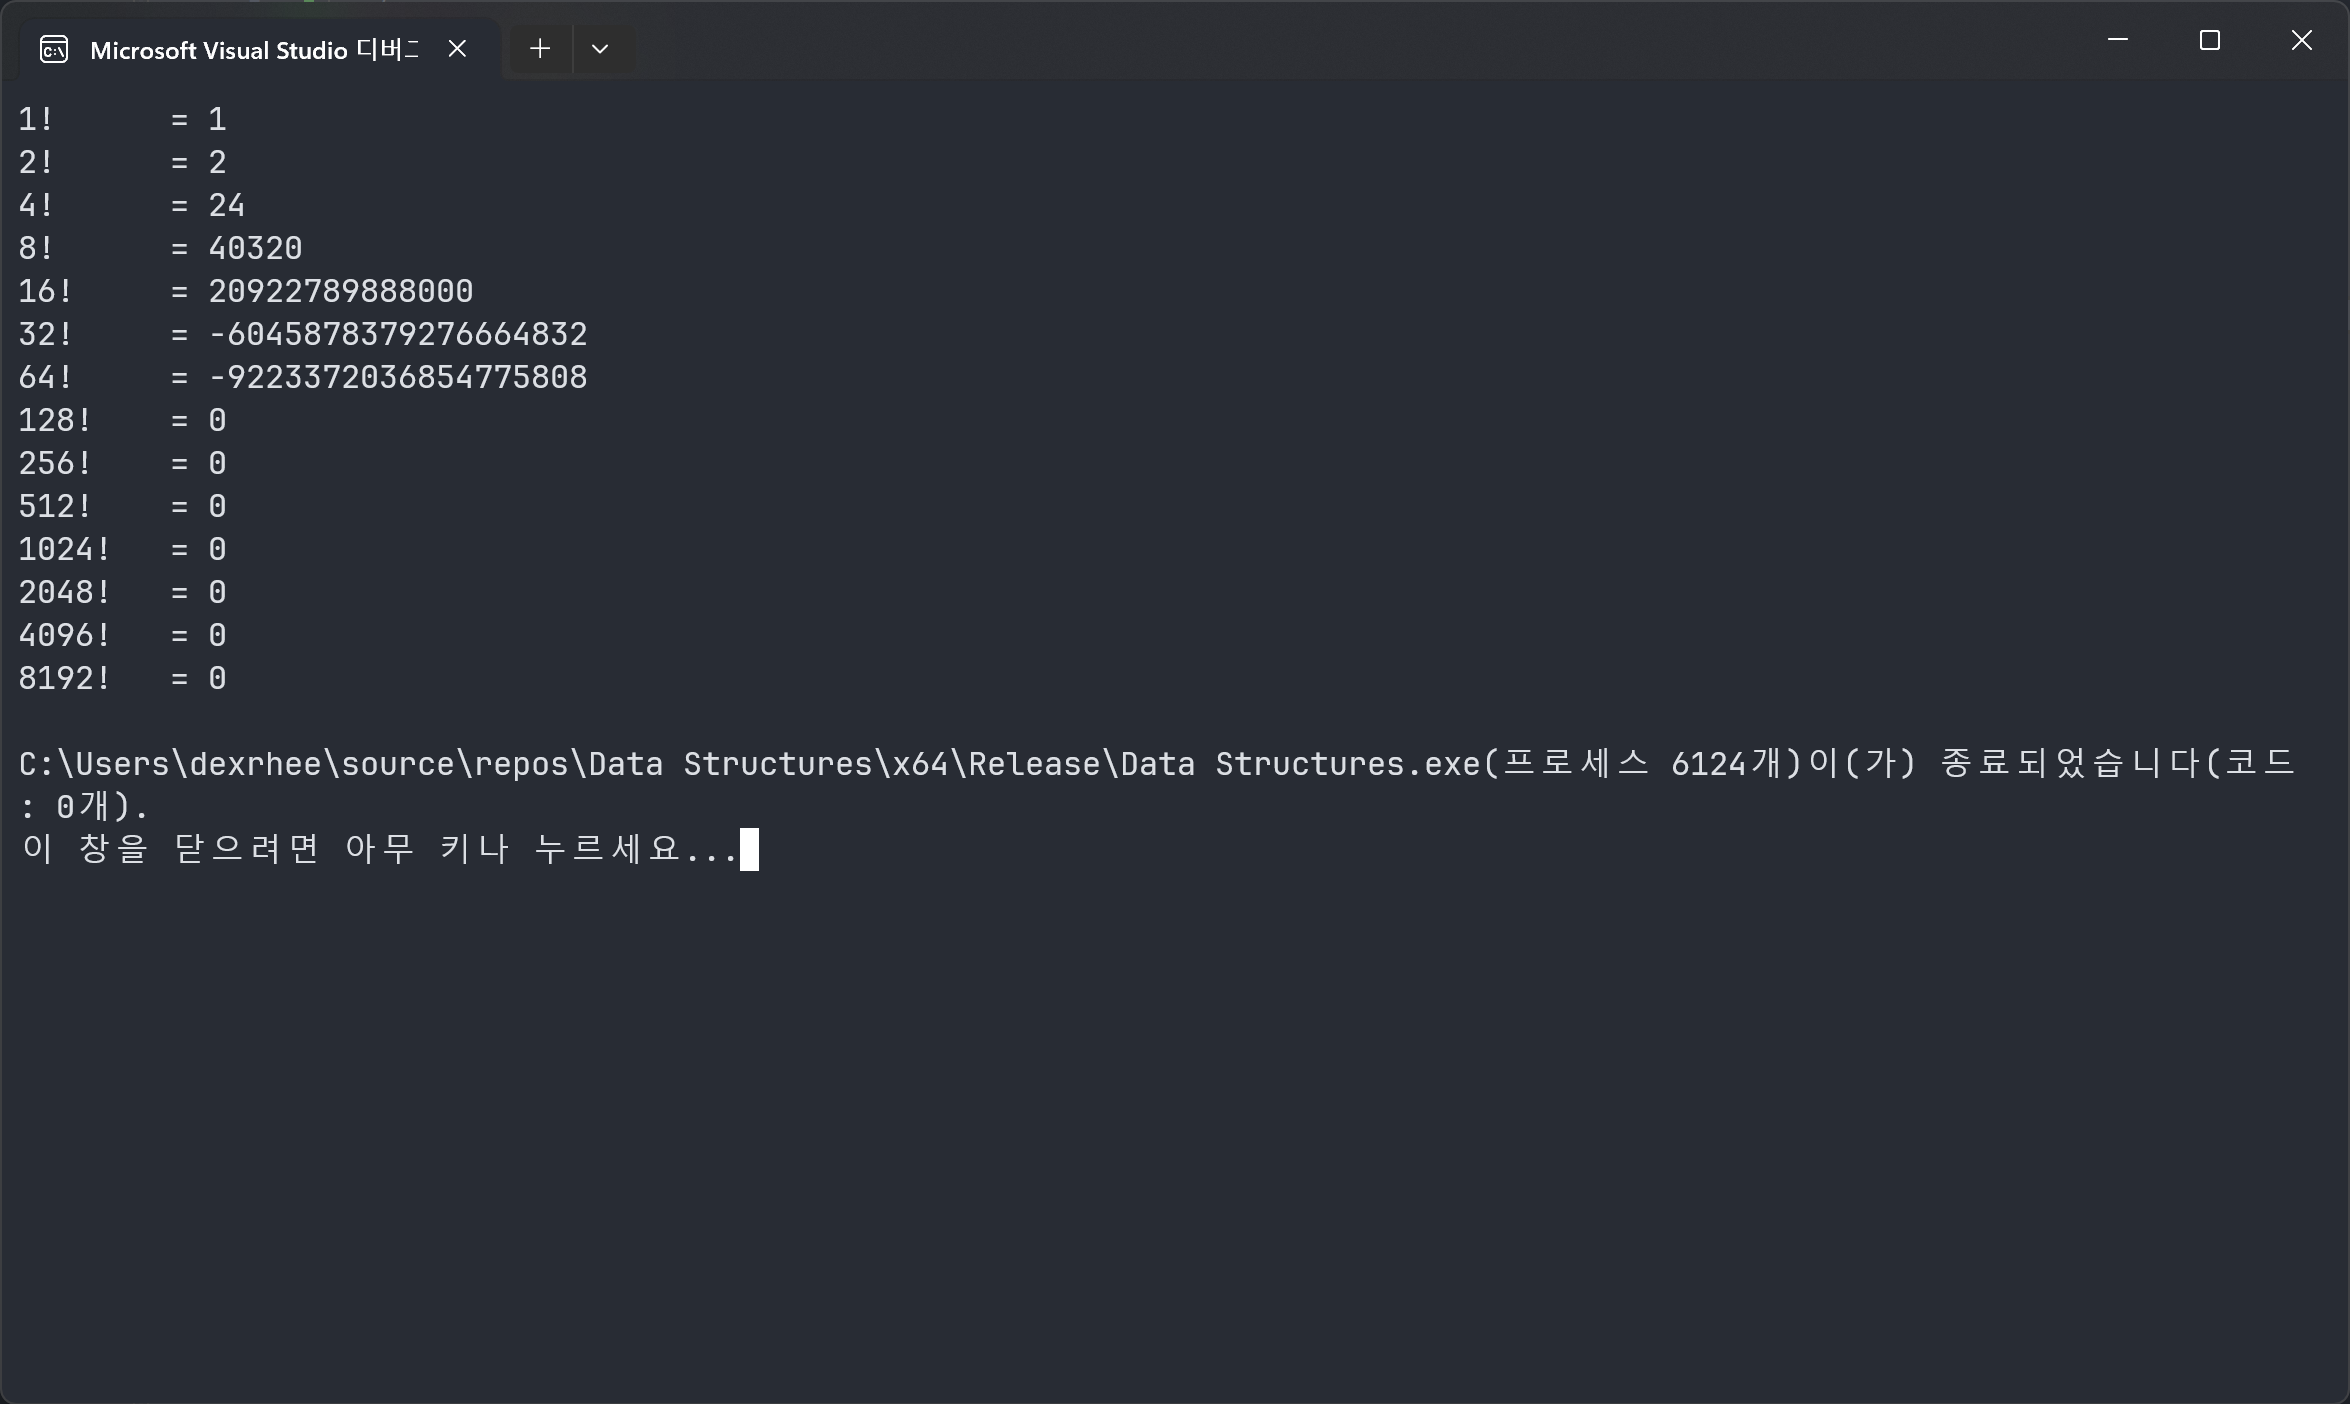
\includegraphics[width=\textwidth]{./img/5-4.png}

따라서 Release 모드로 프로젝트를 Build 하였을 때, 내부적으로 최적화가 이루어져 Stack Overflow가 일어나지 않음을 알 수 있겠습니다.

\subsubsection{실험 환경}\phantom{}\\
본 실험은 다음과 같은 환경에서 진행되었으며, 실행을 진행하는 환경에 따라 위의 내용과 상이할 수 있습니다.

\begin{tabularx}{\textwidth}{l|X}
    \hline
    프로세서 & Intel(R) Core(TM) i7-1165G7 @ 2.80GHz  1.69GHz          \\
    RAM  & 16.0GB                                                  \\
    OS   & Windows 11 22H2(22621.1265)                             \\
    IDE  & Microsoft Visual Studio Community 2022 (64-bit) v17.5.2 \\
    \hline
\end{tabularx}

\subsubsection{참고 문헌}\phantom{}\\
1. all-young, 메모리의 구조 (코드, 데이터, 힙, 스택 영역), 티스토리 블로그, 2020년 9월 4일 작성, 2023년 3월 20일 조회 (https://all-young.tistory.com/17)

2. 코딩팩토리, {[IDE]} 비주얼 스튜디오 Release, Debug 모드의 차이점, 티스토리 블로그, 2021년 1월 24일 작성, 2023년 3월 20일 조회 (https://coding-factory.tistory.com/648)

\end{document}
